%%%%%%%%%%%%%%%%%%%%%%%%%%%%%%%%%%%%%%%%%
% Journal Article
% LaTeX Template
% Version 1.3 (9/9/13)
%
% This template has been downloaded from:
% http://www.LaTeXTemplates.com
%
% Original author:
% Frits Wenneker (http://www.howtotex.com)
%
% License:
% CC BY-NC-SA 3.0 (http://creativecommons.org/licenses/by-nc-sa/3.0/)
%
%%%%%%%%%%%%%%%%%%%%%%%%%%%%%%%%%%%%%%%%%
%----------------------------------------------------------------------------------------
%       PACKAGES AND OTHER DOCUMENT CONFIGURATIONS
%----------------------------------------------------------------------------------------
\documentclass[paper=letter, fontsize=12pt]{article}
\usepackage[spanish]{babel} % Spanish language/hyphenation
\usepackage{amsmath,amsfonts,amsthm} % Math packages
\usepackage[utf8]{inputenc}
\usepackage{float}
\usepackage{lipsum} % Package to generate dummy text throughout this template
\usepackage{blindtext}
\usepackage{graphicx}
\graphicspath{{../media/}}	% Media path
\usepackage{caption}
\usepackage{subcaption}

\usepackage{tikz}
\usepackage{gantt}


\usepackage[sc]{mathpazo} % Use the Palatino font
\usepackage[T1]{fontenc} % Use 8-bit encoding that has 256 glyphs
\linespread{1.05} % Line spacing - Palatino needs more space between lines
\usepackage{microtype} % Slightly tweak font spacing for aesthetics
\usepackage[hmarginratio=1:1,top=32mm,columnsep=20pt]{geometry} % Document margins
\usepackage{multicol} % Used for the two-column layout of the document
%\usepackage[hang, small,labelfont=bf,up,textfont=it,up]{caption} % Custom captions under/above floats in tables or figures
\usepackage{multirow}

\usepackage{booktabs} % Horizontal rules in tables
\usepackage{float} % Required for tables and figures in the multi-column environment - they need to be placed in specific locations with the [H] (e.g. \begin{table}[H])
\usepackage{hyperref} % For hyperlinks in the PDF
\usepackage{lettrine} % The lettrine is the first enlarged letter at the beginning of the text
\usepackage{paralist} % Used for the compactitem environment which makes bullet points with less space between them
\usepackage{abstract} % Allows abstract customization
\renewcommand{\abstractnamefont}{\normalfont\bfseries} % Set the "Abstract" text to bold
\renewcommand{\abstracttextfont}{\normalfont\small\itshape} % Set the abstract itself to small italic text
\usepackage{titlesec} % Allows customization of titles

\renewcommand\thesection{\Roman{section}} % Roman numerals for the sections
\renewcommand\thesubsection{\Roman{subsection}} % Roman numerals for subsections

\titleformat{\section}[block]{\large\scshape\centering}{\thesection.}{1em}{} % Change the look of the section titles
\titleformat{\subsection}[block]{\large}{\thesubsection.}{1em}{} % Change the look of the section titles
\newcommand{\horrule}[1]{\rule{\linewidth}{#1}} % Create horizontal rule command with 1 argument of height
\usepackage{fancyhdr} % Headers and footers
\pagestyle{fancy} % All pages have headers and footers
\fancyhead{} % Blank out the default header
\fancyfoot{} % Blank out the default footer

\fancyhead[C]{Procesador con pipeline $\bullet$ Julio 2015 $\bullet$ IE521} % Custom header text

\fancyfoot[RO,LE]{\thepage} % Custom footer text
%----------------------------------------------------------------------------------------
%       TITLE SECTION
%----------------------------------------------------------------------------------------
\title{\vspace{-20mm}\hrule\vspace{5mm}\fontsize{24pt}{10pt}\selectfont\textbf{Procesador con pipeline de cinco etapas}} % Article title
\author{
\large
\href{mailto:josepabloapu@gmail.com}{\textsc{Jose Pablo Apú, B10407}}\\\href{mailto:marco.torres.810@gmail.com}{\textsc{Marco Torres, B16592}}\\\href{mailto:}{\textsc{Chuan Wu, B27371}} \\[2mm]
%\thanks{A thank you or further information}\\ % Your name
%\normalsize \href{mailto:marco.torres.810@gmail.com}{marco.torres.810@gmail.com}\\[2mm] % Your email address
\normalsize Estructuras de Computadores Digitales II \\[1mm] % Your institution
\normalsize Escuela de Ingeniería Eléctrica \\ % Your institution
\normalsize Universidad de Costa Rica \\ % Your institution
}
\date{}

%----------------------------------------------------------------------------------------
\begin{document}

\maketitle 
\hrule
%%%%%%%%%%%%%%%%%%%%%%%%%%%%%%%%%%%%%%%%%%%%%%%%%%%%%%%%%%%%% 
\begin{abstract}
En este documento se describe detalladamente el diseño, la implementación de un procesador con pipeline de cinco etapas.   
\end{abstract}

%%%%%%%%%%%%%%%%%%%%%%%%%%%%%%%%%%%%%%%%%%%%%%%%%%%%%%%%%%%%%
\section{Introducción}

\subsection{Desarrollo del proyecto}

Se pretende describir un microprocesador con pipeline de cinco etapas. Las características principales son:

\begin{enumerate}
\item No tendrá direccionamiento indirecto.
\item Tendrá dos registros de uso general, llamados A y B.
\item No se harán operaciones de A con Memoria, ni de B con Memoria, únicamente entre A, B y constantes.
\item La memoria de datos estará separada de la de instrucciones.
\item Cada posición de la memoria de datos guardará un byte.
\item Cada posición de la memoria de instrucciones guardará dos bytes.
\item La memoria de datos tendrá 1024 posiciones (10 bits para indexarla).
\item La memoria de instrucciones tendrá 1024 posiciones (10 bits para indexarla).
\item No habrá subrutinas.
\item No se implementará atención a interrupciones.
\item No se implementará una pila.
\item Se supondrán únicamente números sin signo, por lo que no habrá bandera de rebase.
\end{enumerate}

\subsection{Plan de pruebas}

Con la tabla de instrucciones, que se pueden observar en el cuadro \ref{tablaDecodificacion}, se piensa contruir pogramas pequeños, pero característicos, esto para observar el comportamiento del microprocesador.

\section{Diseño}

El que tenga un pipeline, permite estar ejecutando una intrucción, y que en ese momento pueda recibir otra intrucción. Sabemos que las intrucciones por lo general, necesitan de 2 a 3 ciclos de reloj. La idea es que al ejecutarse el segundo ciclo de reloj, el procesador pueda recibir la siguiente instrucción, sin que la primera instrucción finalice. Para lograr esto hay que tener mucho cuidado con el cableado de los módulos.

\subsection{Unidad de control}
El microprocesador tiene una unidad de control, que es este caso se llama decodificador. Este permite administrar las entradas que recibe la alu, los regirstros y además maneja los saltos del microprocesador.

\subsubsection{Estados}



\subsubsection{Entradas}

\subsubsection{Salidas}

\pagebreak
\subsubsection{Definición de la máquina}

\subsection{Multiplexores}

\begin{table}[h]
\centering
\begin{tabular}{cc|cc}
\multicolumn{4}{c}{Sistema de control} \\ \hline
selM1 & selM2 & ln1 	& ln2  \\ \hline
0     & 0     & wA 	& imdt \\
0     & 1     & wA	& wB   \\
1     & 0     & imdt	& imdt \\
1     & 1     & imdt	& wB   \\
\end{tabular}
\end{table}

\subsection{Acumulador}

\begin{table}[h]
\centering
\begin{tabular}{c|c}
\multicolumn{2}{c}{Sistema de control} \\ \hline
selX   & wX    \\ \hline
00     & wX    \\
01     & inmdt \\
10     & alu   \\
11     & mem   \\
\end{tabular}
\end{table}


\pagebreak
\subsection{Decodificador}

\begin{itemize}
\item \textbf{Entradas:}\\
instr
\item \textbf{Salidas:}\\
selA, selB, selM1, selM2, inm, memDir, branchDir, jmpDir, jmpTaken, wrEnable, opCode
\item \textbf{Asignaciónes:} \\
inm = instr[0:7] \\
memDir = jmpDir = instr[0:9] \\
branchDir = instr[0:5] \\
opCode = instr[10:15]
\end{itemize}

En la tabla \ref{tablaDecodificacion} se observa las salidad de control, que hace el decodificador para manejar los registros y los muxes que van hacia la alu.

\begin{table}
\centering
\begin{tabular}{cc|ccccc}
\multicolumn{7}{c}{Salida según la intrucción} \\ \hline
Codificación& Mnemónico	  	& selA & selB & selM1 & selM2 & wrEnable \\ \hline
000 000 	& LDA 		  	& 11 	& 00    & X     & X     & 0 \\
000 001		& LDB  			& 00 	& 11    & X     & X     & 0 \\           
000 010 	& LDCA 			& 01 	& 00    & X     & X     & 0 \\            
000 011 	& LDCB 			& 00 	& 01    & X     & X     & 0 \\           
000 100 	& STA  	 		& 00 	& 00    & 0     & X     & 1 \\            
000 101 	& STB  			& 00 	& 00    & X     & 0     & 1 \\            
000 110 	& ADDA			& 10 	& 00    & 0     & 1     & 0 \\
000 111 	& ADDB			& 00 	& 10    & 0     & 1     & 0 \\
001 000 	& ADDCA			& 10 	& 00    & 0     & 0     & 0 \\
001 001 	& ADDCB			& 00 	& 10    & 1     & 1     & 0 \\
001 010 	& SUBA			& 10 	& 00    & 0     & 1     & 0 \\
001 011 	& SUBB			& 00 	& 10    & 0     & 1     & 0 \\
001 100 	& SUBCA			& 10 	& 00    & 0     & 0     & 0 \\
001 101 	& SUBCB			& 00 	& 10    & 1     & 1     & 0 \\
001 110 	& ANDA			& 10 	& 00    & 0     & 1     & 0 \\
001 111 	& ANDB			& 00 	& 10    & 0    	& 1     & 0 \\
010 000 	& ANDCA			& 10 	& 00    & 0     & 0     & 0 \\
010 001 	& ANDCB			& 00 	& 10    & 1     & 1     & 0 \\
010 010 	& ORA			& 10 	& 00    & 0     & 1     & 0 \\
010 011 	& ORB			& 00 	& 10    & 0     & 1     & 0 \\
010 100 	& ORCA			& 10 	& 00    & 0     & 0     & 0 \\
010 101 	& ORCB			& 00 	& 10    & 1     & 1     & 0 \\
010 110 	& ASLA			& 10 	& 00    & X     & X     & 0 \\
010 111 	& ASRA			& 10 	& 00    & X     & X     & 0 \\
	
011 000 	& JMP			& 00 	& 00    & X     & X     & 0 \\
011 001 	& BAEQ			& 00 	& 00    & X     & X     & 0 \\
011 010 	& BANE			& 00 	& 00    & X     & X     & 0 \\
011 011 	& BACS			& 00 	& 00    & X     & X     & 0 \\
011 100 	& BACC			& 00 	& 00    & X     & X     & 0 \\
011 101 	& BAMI			& 00 	& 00    & X     & X     & 0 \\
011 110 	& BAPL			& 00 	& 00    & X     & X     & 0 \\
011 111 	& BBEQ			& 00 	& 00    & X     & X     & 0 \\
100 000 	& BBNE			& 00 	& 00    & X     & X     & 0 \\
100 001 	& BBCS			& 00 	& 00    & X     & X     & 0 \\
100 010 	& BBCC			& 00 	& 00    & X     & X     & 0 \\
100 011 	& BBMI			& 00 	& 00    & X     & X     & 0 \\
100 100 	& BBPL			& 00 	& 00    & X     & X     & 0 \\

100 101 	& NOP			& 00 	& 00    & X     & X     & 0 \\

\end{tabular}
\caption{Salidas de control, del decodificador}
\label{tablaDecodificacion}
\end{table}


\subsection{Memoria de datos}

\subsection{Memoria de instrucciones}

%%%%%%%%%%%%%%%%%%%%%%%%%%%%%%%%%%%%%%%%%%%%%%%%%%%%%%%%%%%%%
\section{Implementación}

\begin{figure}[hbtp]
\centering
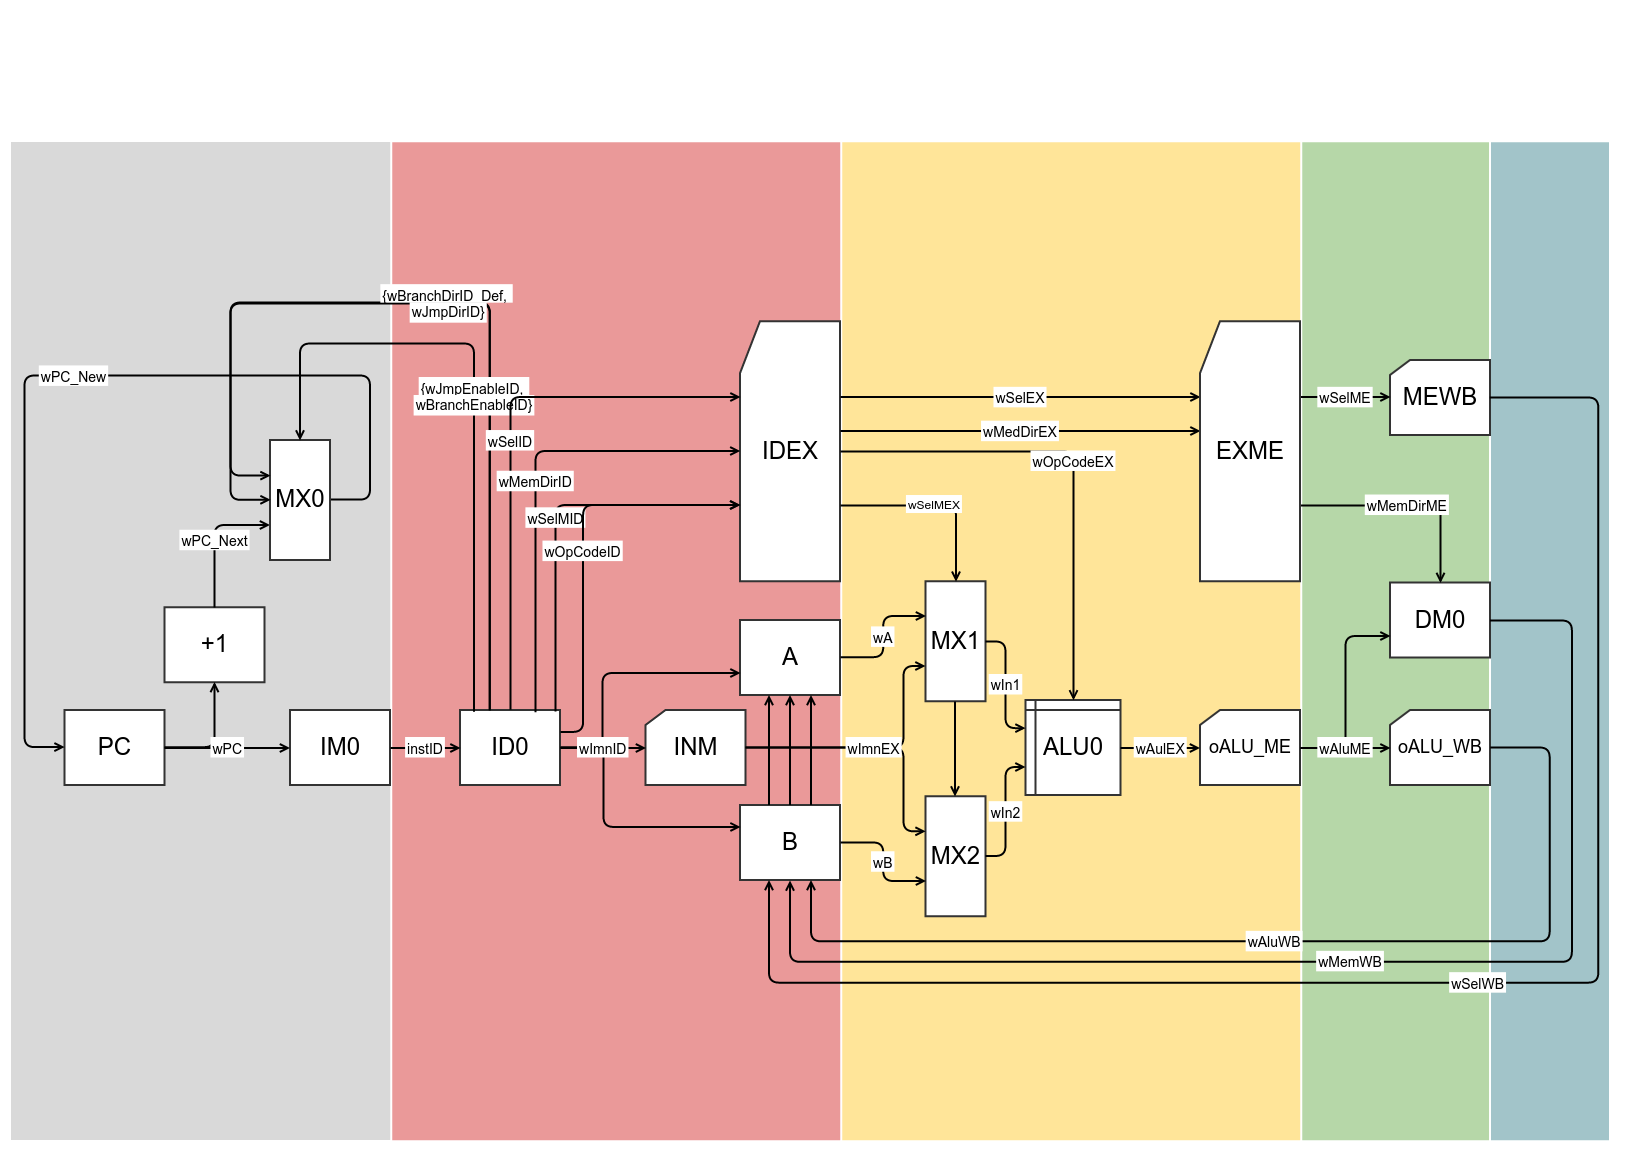
\includegraphics[width=1\linewidth]{diagramaBLoques.png}
\caption{Plan de pruebas}
\end{figure}

%%%%%%%%%%%%%%%%%%%%%%%%%%%%%%%%%%%%%%%%%%%%%%%%%%%%%%%%%%%%%
\section{Verificación y plan de pruebas}

Primero se cargo un LDCA y un LDCB. Luego se sumaron con una ADDA y finalmente se guardó en memoria con un STA.

\begin{figure}[hbtp]
\centering
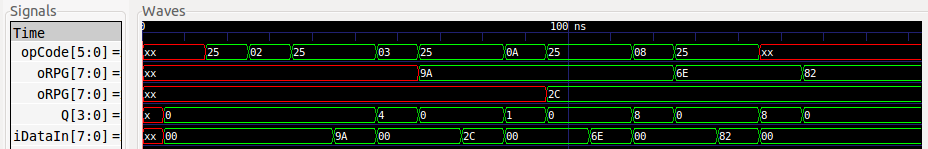
\includegraphics[width=1\linewidth]{planPruebasUno.png}
\caption{Plan de pruebas}
\end{figure}

EN otra prueba.. CHUAN AQUÍ VA UNA SUYA
\end{document}
